%Acá explicamos cómo extrajimos los datos, qué características tiene la muestra (muchos de los análisis/gráficos ya los hicimos), cómo la separamos, y qué análisis estadísticos estamos realizando (es la parte que nos falta)


\section{Extracción de Datos}

Para la recolección de tweets, primero se extrajo una cantidad de usuarios de forma localizada con el fin de obtener todos los tweets de estos.
Los usuarios se buscaron por provinicia de modo tal que haya una cantidad aproximadamente equitativa.
La búsqueda de los usuarios se hizo de la siguiente manera:

Por cada provincia de la Argentina, se extrajo las ubicaciones de cada uno de sus departamentos , de los partidos de la provincia de Buenos Aires y de las comunas de la Ciudad Autónoma de Buenos Aires. El conjunto de estas forman la subdivisión de segundo orden de la republica Argentina. La lista de departamentos/partidos/comunas fue extraída a partir de los datos publicados del Censo Argentino realizado en el año 2010. Para extraer los tweets se utilizó la librería de \textit{python} llamada \textit{tweepy}.
De esta manera se recolectó aproximadamente 2000 usuarios por provincia lo que resume en 46000 usuarios argentinos. Sobre este conjunto de usuarios se buscaron los tweets realizados por estos. Se decidió no tener en cuenta los retweets dado que estos no son escritos por los usuarios sino que son una mera copia de otros tweets. 


\subsection{Búsqueda geolocalizadas}

Las búsquedas geolocalizadas de la API de \textit{twitter} primero intentan de buscar tweets cuyas coordenadas sean las buscadas. En caso de no tener éxito, buscará aquellos tweets creados por usuarios que tienen en el campo \textit{location} de su perfil un lugar cuyo geocódigo coincida con el de sus coordenadas. Es decir, si se hace una búsqueda inversa de las coordenadas, devuelve el lugar de su perfil.

Una vez obtenida la lista de ubicaciones, se realizaron búsquedas por cada provincia con centro en las coordenadas de los departamentos de la misma y con un radio de 20 millas. Sobre el resultado de esta búsqueda, únicamente se seleccionaron los usuarios que tienen como campo \textit{location} al menos uno de los nombres de las ciudades de la provincia. Con esta precaución eliminamos los posibles tweets de turistas que escribieron en un lugar pero que no viven allí.

En el gráfico de la figura \ref{fig:busqueda_usuarios} se muestran las ubicaciones donde se encuentran los usuarios de la muestra de desarrollo:

\begin{figure}[ht]
\centering
% \includegraphics[scale=0.6]{imagenes/ubicacion_usuarios.png}
\caption{Ubicaciones de los usuarios} 
\label{fig:busqueda_usuarios} 
\end{figure}

Si bien en este trabajo nos enfocamos en las coordenadas de las localidades dentro de Argentina, basta con cambiar las coordenadas y los nombres de las localidades que tienen que tener los campos \textit{location} para realizar un análisis sobre otros países.


\section{Datos de desarrollo y de validación}

Por cada provincia se tomó a los usuarios de la misma y se los dividió para tener un conjunto de datos de desarrollo y uno de validación. El conjunto de validación fue creado para poder corroborar que los resultados obtenidos por el análisis del conjunto de desarrollo no sean algo intrínseco de esta muestra, sino que se pueden extrapolar a toda la población. 
La división de los datos se realizó de manera tal que los conjuntos resultantes sean lo más independientes posibles: 
\begin{description}
    \item [Usuarios disjuntos] Debido a que ciertos usuarios repiten palabras constantemente, ya sea porque son bots o simplemente porque hablan siempre de los mismos temas, es adecuado validar los resultados con textos producidos por distintos usuarios. De esta manera se intentó mitigar el ruido generado por estos usuarios particulares.
    \item [Fechas disjuntas] Al analizar los resultados sobre los textos generados en un tiempo acotado de tiempo, estamos trabajando con una muestra específica que es de esperar que tenga fenómenos particulares debido al momento en que fueron escritos. Por ejemplo, debido a cierto fenómeno climático o en el transcurso de un evento polémico (como un debate presidencial o un torneo deportivo) se pueden obtener tweets con una frecuencia de ciertas palabras muy distinta a la frecuencia de la población. Por esta razón se dividió los tweets producidos por los usuarios de manera tal que sus fechas sean disjuntas.
\end{description}

La división fue de la siguiente manera:
Sobre el conjunto de usuarios se dividió en dos de forma aleatoria, obteniendo $Usuarios_1$ y $Usuarios_2$. Luego se buscó la fecha $Fecha_{DIV}$ por la cual había una cantidad equiparable entre el conjunto de tweets producidos por  $Usuarios_1$ antes de $Fecha_{DIV}$ y el conjunto de tweets producidos por $Usuarios_2$ despúes de $Fecha_{DIV}$.Es decir:

\begin{equation}
%\sum_{ f = FechaInicial}^{Fecha_{Div}} tweets(Usuarios_1,f) \approx \sum_{ f = Fecha_{Div}}^{FechaFinal} tweets(Usuarios_2,f) 
 Fecha_{DIV}  = \operatorname*{arg\,min}_{F} \left|\sum_{ f = FechaInicial}^{F} tweets(Usuarios_1,f) - \sum_{ f = F}^{FechaFinal} tweets(Usuarios_2,f)\right|
\end{equation}

Después de fijar la fecha se dividió al conjunto de tweets producidos por estos usuarios: el conjunto de desarrollo con los tweets producidos antes de $Fecha_{DIV}$ y el conjunto de test producidos posteriormente a esa fecha.

\section{Tokenización y normalización}


En cuanto al análisis del texto surge una primer problemática: ¿qué es una palabra?. En principio podemos definir a una palabra como cualquier secuencia de caracteres delimitados por espacios blancos. Con esta definición 523456 y ? serían palabras. Debido a esto podemos restringir nuestra definición a una secuencia de caracteres alfabéticos. Ahora los ejemplos mencionados anteriormente dejarían de estar dentro de la definición. Sin embargo términos como asdsdafsdf también serían palabras. Para restringir aún más la definición podríamos tener un diccionario como filtro para saber si una secuencia de caracteres dada es una palabra. Si bien esto tendría mucha precisión al momento de filtrar los términos, no seríamos capaces de palabras que existen en un lenguaje pero que no están representadas bajo el diccionario elegido. Es por eso que decidimos tomar a una palabra como una secuencia de caracteres alfabéticos.

Es muy posible que tengamos palabras que no sean interesantes a nivel lingüistico, como errores de tipeo (e.g computadira, escribur), errores ortográficos o  nombres propios. Es importante destacar que Twitter tiene caracteres especiales para mencionar a la gente, como el @, o el \#(hashtag) utilizado para agrupar mensajes. Estos caracteres aparecen mucho, ya que los usuarios suelen responderse en la red, mencionando los mismos temas (aclarando el hashtag), o respondiendo a otros usuarios. Ya que esos caracteres no son alfabéticos, cualquier término que los utilice no va a ser parte del conjunto de palabras, como tampoco lo serán las direcciones de páginsa web. Decidimos que se filtren estos terminos ya que no tienen interés lingüistico y además agregarían mucho ruido a los datos.

Además de la tokenización del texto, se realizó una normalización sobre él. Todas las letras se convirtieron a letra minúscula y las palabras con más de tres letras iguales de forma consecutiva se redujeron para que solo tengan tres repeticiones. De esta forma, el término \textit{padreeeee} y \textit{padreeee} fueron reducidos a una única unidad léxica (\textit{padreee}). Esto se realizó con la librería \textit{TweetTokenizer de NLTK}. 
Se descartó la idea de filtrar las palabras que no estuvieran en un diccionario ya que si bien hubiera eliminado mucho ruido, también nos hubiera filtrado palabras de interés. Este es el caso de los neologismos, o las palabras que si bien se utilizan hace mucho tiempo no están en los diccionarios actuales.

\section{Caracterización de la muestra}

Para tener una noción más completa de la muestra, se peresenta en la tabla \ref{tab:cantidades} la cual indica las cantidades de palabras y tweets por provincia.


\begin{table}[ht]
\centering

\label{tab:cantidades}
\begin{tabular}[width=0.7\textwidth]{|l|c|c|c|c|c|c|}
\hline
Provincia      & \#Palabras Distintas & \#Usuarios & \#Tweets & \#Total Palabras \\ \hline
Buenos Aires   & 191919       & 920          & 1125042    & 8974372  \\
Catamarca      & 173104       & 957          & 1057019    & 8161309   \\
Chaco          & 169476       & 964          & 976943     & 7605991   \\
Chubut         & 182592       & 954          & 1023373    & 8884745   \\
Córdoba        & 207307       & 987          & 1224266    & 10075932  \\
Corrientes     & 183292       & 939          & 1044951    & 8426940   \\
Entre Ríos     & 188679       & 969          & 1193693    & 9462986  \\
Formosa        & 169254       & 903          & 923352     & 7184382   \\
Jujuy          & 171064       & 971          & 678004     & 5951778   \\
La Pampa       & 186593       & 935          & 1085757    & 8996318  \\
La Rioja       & 186041       & 946          & 704044     & 6757277  \\
Mendoza        & 193708       & 945          & 1099717    & 9402399   \\
Misiones       & 168400       & 972          & 984218     & 7790197   \\
Neuquén        & 188038       & 927          & 1111201    & 9021449   \\
Río Negro      & 194383       & 965          & 1215361    & 9991831  \\
Salta          & 188402       & 884          & 830916     & 7506652   \\
San Juan       & 183546       & 926          & 1002322    & 8377792  \\
San Luis       & 164185       & 896          & 1006464    & 8327093  \\
Santa Cruz     & 174089       & 935          & 876621     & 7432923  \\
Santa Fe       & 201879       & 937          & 1019620    & 8862328  \\
Santiago del Estero       & 166540       & 887          & 944109     & 7355729  \\
Tierra del Fuego & 197273       & 964          & 976426     & 8559218   \\
Tucumán        & 195643       & 962          & 1093874    & 9238526 \\
  \hline
\end{tabular}
\caption{Cantidades del conjunto de datos de desarrollo}
\end{table}



\subsection{Cantidad de palabras}
%Cantidad de palabras promedio por tweet
%Cantidad de palabras por usuario + varianza por provincia
\subsection{Tweets a lo largo del tiempo}
Los tweets recolectados para el conjunto de datos de desarrollo tienen una particularidad: a médida que pasan los años 
hubo mayor cantidad de tweets durante un año. Esto se refleja en los gráficos de las figuras \ref{fig:histTweetsProvincia1} y \ref{histTweetsProvincia2}.

\begin{figure}[!ht]\centering
   \begin{minipage}{0.49\textwidth}
     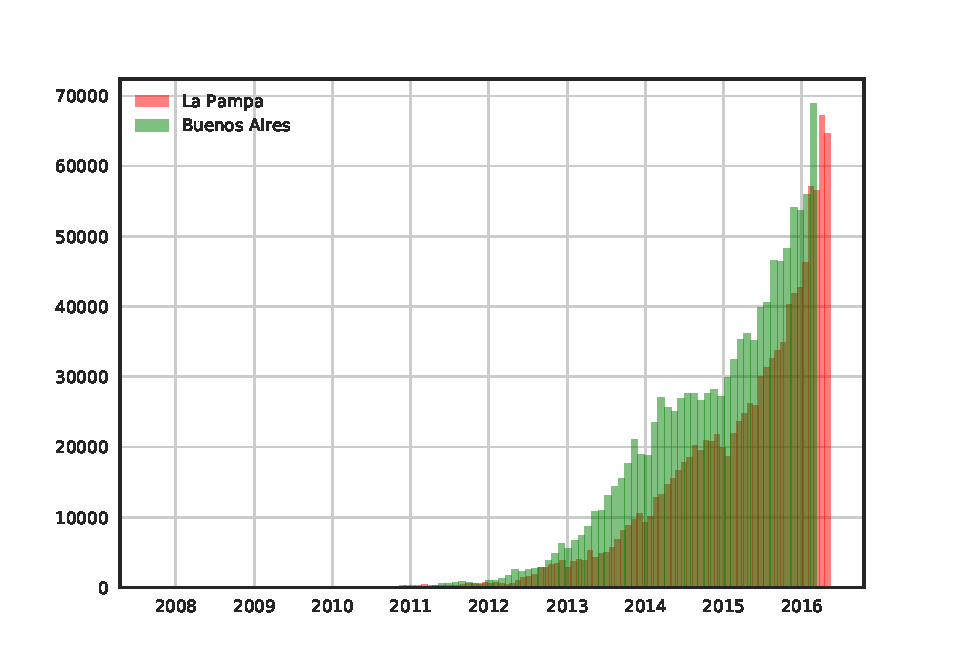
\includegraphics[width=\linewidth]{./images/train/sinFiltro/histTweetsProvincia1_sinFiltro.pdf}
     \caption{}
     \label{fig:histTweetsProvincia1}
   \end{minipage}
   \begin {minipage}{0.49\textwidth}
     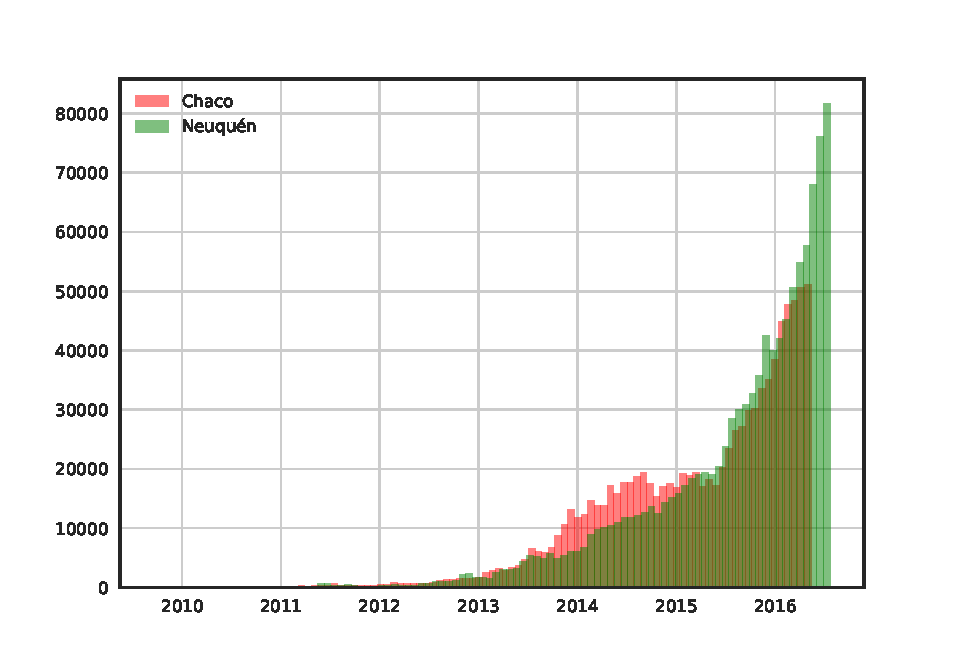
\includegraphics[width=\linewidth]{./images/train/sinFiltro/histTweetsProvincia2_sinFiltro.pdf}
     \caption{}
     \label{fig:histTweetsProvincia2}
   \end{minipage}
   \caption { En la figura \ref{fig:histTweetsProvincia1} se presenta un histograma donde se muestra la cantidad de tweets que se hiceron por intervalo de tiempo en la provincias La Pampa y Buenos Aires. En la figura \ref{fig:histTweetsProvincia2}, se presenta el gráfico para Chaco y Neuquén.}
\end{figure}


% Tweets promedio por usuario, por provincia. (varianza)

% cantidad de tweets por usuario, cantidad media de palabras por usuario

\section{Búsqueda de contrastes}

% Definir que es un contraste, que tiene un uso significativo en una region más que en otra. LAs alternativas que propusimos, z test binomial.
Diremos que una palabra tiene un contraste cuando esta tiene un uso con diferencias significativas en
distintas regiones. En este trabajo nos propusimos crear un listado con palabras con contrastes que tengan
importancia a nivel lingüistico. En este sentido, los nombres de personas, lugares u organizaciones no 
fueron considerados de interés a pesar de tener contrastes en su uso.
Este listado fue ordenado por una métrica que capte en un único valor el nivel contrastivo. De esta manera, 
se seleccionó un subconjunto de palabras, de acuerdo a la métrica, el cual fue analizado manualmente en otros textos por la Academia Argentina de Letras.

El primer acercamiento para ver el contraste de las palabras lo realizamos comparando las frecuencias de las palabras 
en cada par de prinvincias de la Argentina. Para esto calculamos el cociente entre la frecuencia máxima de la palabra
en las dos provincias sobre la frecuencia mínima, al que llamaremos \textit{maxDif}. En caso de que en una de las dos provincias no se haya 
recolectado tweets con esa palabra, se tomaba como frecuencia mínima a la frecuencia mínima distinta de 0 de todas las palabras generadas en esa provincia. Así se evitó la división por cero.
De esa manera se ordenó el listado de cada par de provincias teniendo en cuenta la división de frecuencias. 
Sin embargo, este método imposibilitaba el trabajo manual para la Academia Argentina de Letras que debía mirar estos listados y hacer un análisis más exhaustivo sobre las palabras con mayor diferencia de frecuencias, debido a que había $\binom{23}{2} = 253$
listados (o equivalentemente 253 columnas en un mismo listado) a analizar. Además la métrica solo permitía saber si había un contraste entre dos provincias, pero no se podía tener en cuenta la frecuencia de la palabra en el resto de las provincias. 
% Mencionar que la idea era realizar un z test para obtener las palabras más significativas.
En consecuencia las palabras se encontraban repetidas en los distintos listados y con diferentes valores de \textit{maxDif}, lo cual hacía muy díficil poder identificar en que regiones había una diferencia significativa de frecuencias.

Debido a esto decidimos realizar un nuevo enfoque para encontrar las palabras con alta contrastividad en las distintas regiones, de manera que una métrica pueda reflejar el nivel de contrastividad de la palabra en un único valor.
De este modo, nos enfocamos a analizar el contraste de frecuencias de palabras sobre las provincias a través de una métrica superadora.

\subsection{Métricas para medir el contraste en la frecuencia de las palabras}
Dado que se quiere encontrar las palabras con contrastes significativos en distintas 
regiones se propone generar una métrica basada en la cantidad de información 
para poder realizar esta tarea.

Una médida que se puede usar para comparar las frecuencias de las palabras en las difentes regiones del país puede ser la entropía definida por Shannon\ref{sub:entropiaShannon}, debido a que podemos tener un valor que informe que tan uniforme es la distribución de las frecuencias de cada palabra.
Sin embargo, la entropía como única médida tiene sus desventajas. Principalmente, una palabra con una sola ocurrencia en una provincia y ninguna en las demás, tiene la entropía mínima. A pesar de que nos interesan las palabras con un contraste significativo entre regiones, dentro de ellas eligiremos las que tienne mayor cantidad de ocurrencias. Es por esto que elaboramos otra métrica que tenga en cuenta la entropía, pero que no sea la única variable a tener en cuenta.


\subsection{Valor de información}
La métrica que utilizamos para ordenar los listados de palabras y detectar cuales son
las que tienen altos contrastes en su uso en distintas regiones fue inspirada sobre el
trabajo de Zanette y Montemurro \cite{montemurro2010towards}.
Ellos a diferencia de Shannon estudiaron una relación entre una médida de la información y su función semántica en el lenguaje.
A continuación detallamos el procedimiento para calcular lo que ellos llamaron
el valor de la información:

Dado un texto dividido en P partes iguales, se calcula la entropía  $H(w)$ sobre el vector de cantidad de ocurrencias en cada una de las P ventanas.
Luego se define $\widehat{H(w)}$  como la entropía de una permutación aleatoria del texto y promediada por todos las posibles realizaciones de la permutación de él. 
%% CHEQUEAR LA DEFINICION DE LA ENTROPIA SHUFFLEADA

Es decir, se distribuyen uniformemente las palabras en P partes y se calcula la
entropía como se hizo con el texto original. Es de esperar que en la mayoría de casos 
la entropía del texto permutado sea mayor que la médida en el calculo original. Esto 
se debe a que las palabras se distribuyen de forma más uniforme 
en las distintas partes.
Finalmente, definen al valor de la información como $I(w) = p(w) (\widehat{\eta(w)} - \eta(w))$ , con $p(w)$ la frecuencia total de la palabra en el texto. 
De esta manera se le da más importancia a las palabras que son más frecuentes y a las palabras que tienen una baja entropía, ya que en estas el término de la diferencia es más grande.
Este estudio se hizo sobre tres textos, \textit{Análisis de la mente}, 
\textit{Moby Dick} y \textit{El origen de las especies} de Charles Darwin. 
En los tres libros las palabras con mayor valor de la información están 
altamente relacionadas con los temas principales.

Si bien esta métrica tiene en cuenta la frecuencia de las palabras además de la 
entropía, el texto en Twitter resulta dificil dividirlo en partes iguales. 
Esto es porque la división está pensada para dividir al texto en secciones que 
posiblemente hablen de distintos temas y nuestros textos son tweets que por lo general no superan las 10 palabras.
Otra dificultad que surge de esta métrica es la imposibilidad de realizar la media 
de todas las posibles permutaciones del texto por la limitación computacional ya que 
tenemos una cantidad muy grande de datos.

Es por eso que realizamos una métrica parecida:

Podemos pensar a las palabras del texto como una variable aleatoria W, donde cada palabra w tiene una probabilidad de aparición en una provincia dada de la Argentina. Esta probabilidad la aproximamos con la frecuencia en la que aparece, es decir la cantidad de ocurrencias de la palabra dividida por la cantidad de palabras totales.
Por otro lado sea P una variable aleatoria que cuenta la cantidad de personas que 
utilizan la palabra p en cada provincia.

Luego,
\begin{equation}
%I(w) =  norm_{p}(w) * norm_{u}(w) * (\widehat{H}_{w}(w) - H_{w}(w)) * (\widehat{H}_{p}(w) - H_{p}(w)) \\
I(w) =  I_p(w) * I_u(w)\\
\end{equation}
\begin{equation}
I_p(w) = norm_{p}(w) * (\widehat{H}_{w}(w) - H_{w}(w)) \\
\end{equation}
\begin{equation}
I_u(w) = norm_{u}(w) * (\widehat{H}_{u}(u) - H_{u}(w))
\end{equation}

\begin{equation}
norm_{p}(p) = \frac{cw(p)- MIN_W }{MAX_W - MIN_W}
\end{equation}
donde:
\noindent\begin{minipage}{.5\linewidth}
\begin{equation}
  MIN_W = \min\limits_{p \in Palabras} cw(w)
\end{equation}
\end{minipage}%
\begin{minipage}{.5\linewidth}
\begin{equation}
  MAX_W = \max\limits_{p \in Palabras} cw(w)
\end{equation}
\end{minipage}
donde $cw(p)$ es igual al logaritmo sobre la cantidad de ocurrencias de esa palabra en toda la Argentina, es decir $cw(p) = \log_2(cantidadOcurrencias(p))$.

Análogamente,
\begin{equation}
norm_{u}(w) = \frac{cu(w)- MIN_U }{MAX_U - MIN_U}
\end{equation}
\noindent\begin{minipage}{.5\linewidth}
\begin{equation}
  MIN_U = \min\limits_{p \in Palabras} cu(p)
\end{equation}
\end{minipage}%
\begin{minipage}{.5\linewidth}
\begin{equation}
  MAX_U = \max\limits_{p \in Palabras} cu(p)
\end{equation}
\end{minipage}
donde $cu(p)$ es el logaritmo sobre  la cantidad de usuarios que utilizan dicha palabra en la Argentina, es decir $cu(p)= \log_2(cantidadUsuarios(p)))$.
$\widehat{H}$ es la entropía con las cantidades distribuidas uniformemente y H es la entropía común.

Tanto $norm_{w}$ como $norm_{u}$ realizan una normalización del logaritmo de esas variables. Esto se debe a que el logaritmo genera una dispersión en las medidas de forma tal que su distribución sea más uniforme a lo largo de todo el rango de valores. Esto se puede ver en la figura \ref{fig:cantNorms}.
$\widehat{H}_{u}$ y $\widehat{H}_{w}$ se corresponde a las entropías de los vectores simulados de apariciones.
Esta simulación se realiza con una distribución multinomial ya que se distribuye la suma de los valores de la variable aleatoria uniformemente. 

% La variacion de la entropia se puede ver como una cantidad que mide cuanta información se necesita para poder obtener esa distribución
% Si las cantidades de ocurrencias (o de personas que utilizan) de un término están distribuidas uniformemente a través de todas las provincias, quiere decir que no aporta demasiada información 

\begin{figure}[!ht]
\centering
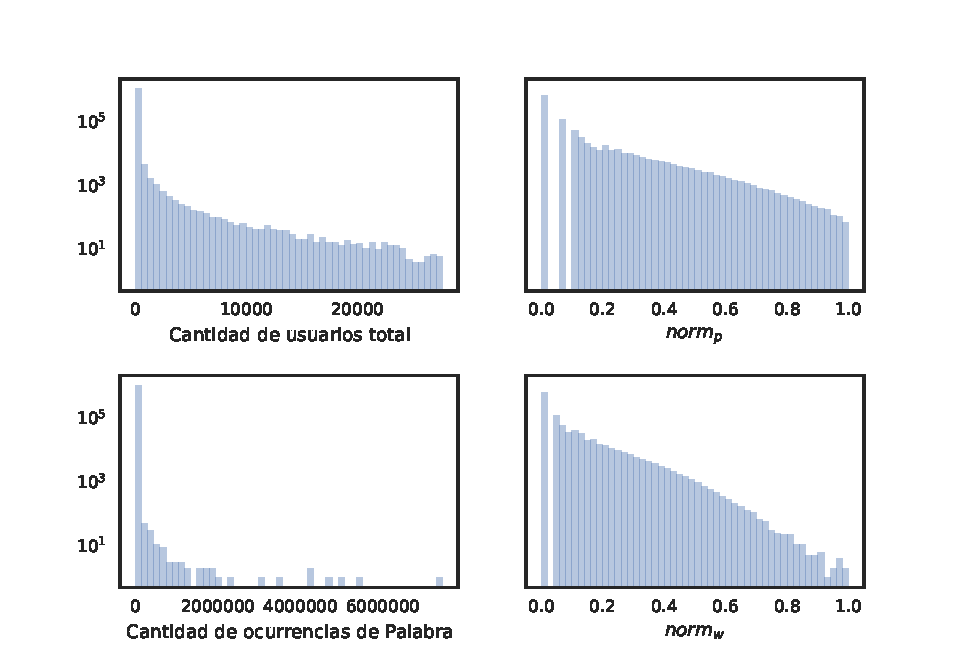
\includegraphics[width=1.0\textwidth]{./images/train/sinFiltro/cantNorms_sinFiltro.pdf}
\caption{Cantidades y sus normalizaciones} 
\label{fig:cantNorms} 
\end{figure}

El término de la diferencia de la entropía sobre la cantidad de personas que utilizan la palabra tiene como objetivo mitigar el ruido de la entropía de palabras. En particular una determinada provincia o región pueden tener muchas ocurrencias de una palabra causado por algunos usuarios que utilizan constantemente el término. Un ejemplo de esto podrían ser bots que escriben automáticamente textos iguales (o similares) en grandes cantidades. Otra posible causa de este fenomeno podría ser la de usuarios de ciertas organizacioenes que hablan de personas, lugares o marcas de forma constante. 
Para eliminar outliers se procedió a eliminar las palabras que tenían una cantidad de usuarios menor o igual a 40 ocurrencias, como también las palabras que eran dichas por menos de 6 personas. 

\subsection{Frecuencia de las palabras}
\label{sub: frecuenciaPalabras}
% Ver si se hace este gráfico con todas las palabras ya que por ahora tengo el conjunto de palabras con más de 40 ocurrencias
En la figura \ref{fog:cantPalabras} graficamos la distribución de la cantidad de ocurrencias de las palabras.Podemos observar que la mayoría de las palabras ocurren poco. En particular el 50\% de las palabras ocurren menos de 139 veces. Por otro lado hay pocas palabras que ocurren mucho, por ejemplo la palabra \textit{que} o la preposición \textit{de}.

\begin{figure}[ht]
\centering
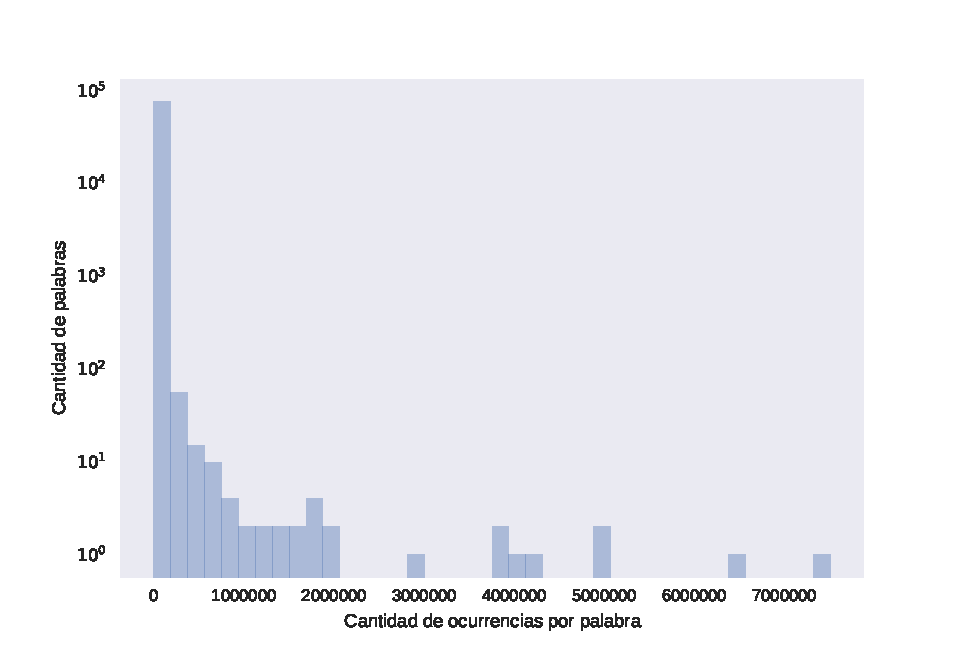
\includegraphics[width=0.8\textwidth]{./images/DistribucionOcurrenciasPalabras.pdf} 
\caption{Histograma de la cantidad de ocurrencias de las palabras} 
\label{fig:cantPalabras} 
\end{figure}

\begin{table}[ht]
\centering
\label{tab:palabrasMasOcurrentes}
\begin{tabular}{|c|c|}
\hline
Palabra & Cantidad de Ocurrencias \\ \hline
que     & 7509160                 \\
de      & 6527014                 \\
a       & 4962492                 \\
la      & 4913854                 \\
no      & 4177810                 \\
me      & 4101998                 \\
y       & 3838370                 \\
el      & 3773455                 \\
en      & 2969783                 \\
te      & 2060662                 \\
se      & 1976027                 \\
un      & 1863075                 \\
es      & 1825892                 \\
con     & 1799979                 \\
lo      & 1712189                 \\
mi      & 1643777                 \\
por     & 1553382                 \\
los     & 1498941                 \\
para    & 1398757                 \\
las     & 1212452                 \\
\hline
\end{tabular}
\caption{Cantidad de apariciones de las 20 palabras más frecuentes}

\end{table}

Si comparamos la posición de la palabra en un listado ordenado podemos ver que se cumple con la ley de Zipf. Esta es una ley empírica formulada por George Zipf en el año 1932 en la cual se establece una relación entre la frecuencia de una palabra con su posición dentro del listado de palabras ordenadas por frecuencia decreciente. En particular, sea $s$ la posición de la palabra en el listado ordenado y sea $f(s)$ la cantidad de ocurrencias de la palabra, se puede hacer la siguiente aproximación:

$$f(s) \approx \frac{A}{s^{\alpha}}$$
donde $\alpha$ toma un valor levemente mayor a 1 y A es una constante.

\begin{figure}[!ht]
\centering
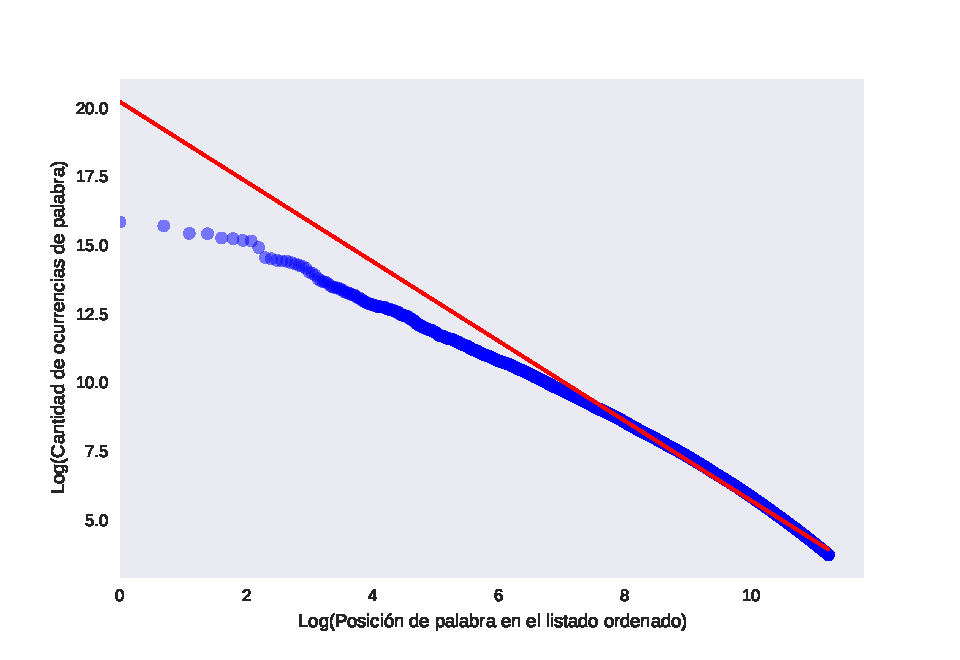
\includegraphics[width=0.5\textwidth]{./images/zipf.pdf}
\caption{Cantidad de Ocurrencias de palabra vs posición en listado ordenado. Se aplicó el logaritmo a las cantidades de ocurrencias, como también a los valores de las posiciones para mostrar la proporcionalidad entre $f(s)$ y $\frac{1}{s^{\alpha}}$} 
\label{fig:zipf} 
\end{figure}


\subsection{Test Hipergeométrico}
Luego de realizar el listado de palabras ordenado por el valor de la información se realizó un test estadístico para tener mayor confianza de que las palabras clasificadas como contrastivas realmente tienen esta propiedad y no fueron producto del azar. Se seleccionó un conjunto de palabras significativas a nivel lingüistico a partir de las 10000 palabras consideradas más contrastivas por nuestra métrica. 

Decidimos elegir el test hipergeométrico ya que querémos ver que la palabra sobre la que se hace el test no estuvo sobrerrepresentada en comparación con la población. Asumimos que la cantidad de ocurrencias de una palabra se puede modelar con una distribución hipergeométrica ya que se puede pensar como un experimento donde se obtuvieron k palabras exitosas en una región con n palabras y un total de N palabras en la Argentina. Las regiones que utilizamos para cada palabra, son el conjunto de provincias que cubren el 80\% de las ocurrencias de dicho término. Luego, queremos calcular la significancia estadística de haber obtenido esas k palabras exitosas.

La hipótesis nula consiste en que la cantidad de ocurrencias de la palabra en la región elegida es mayor a lo observado. 
Por lo tanto, sea  cantPalabrasW(Region) igual a la cantidad de ocurrencias observada de la palabra en la región a analizar.


\begin{table}[ht]
\centering
\label{tab:contingencia}
\begin{tabular}{lccc}
\hline
& \#Palabras Sobre Region &\#Palabras en el resto de Argentina &Total \\ \hline
\# Palabras w &   k & K-k & K \\ 
\# Palabras $\neq$ w & n-k & N + k - n - K  & N - K \\ 
Total & n & N -n & N \\ \hline
\end{tabular}
\caption{Tabla de contingencia}

\end{table}



$$
\begin{cases}
H_0 :  x > cantPalabrasW(Region) \\
H_1 : x \leq cantPalabrasW(Region)
\end{cases}
$$  
siendo x la esperanza de la variable aleatoria que representa la cantidad de palabras exitosas en esa región.
